\noindent {\bf Architecture and assumptions.}
%
We now present our generic \emph{meta}-protocol for information
distribution and retrieval over an interconnection of heterogeneous
overlay networks. Information is a set of basic {\tt (key,value)}
pairs, as commonly encountered in protocols for information retrieval.
The protocol specifies how to insert information ({\tt PUT}), how to
retrieve it through a key ({\tt GET}), how to invite nodes in a given
overlay ({\tt INVITE}), and how to join a given overlay ({\tt JOIN})
over a heterogeneous collection of overlay networks linked by
co-located nodes. These co-located nodes represent a simple way to
aggregate the resources of distinct overlays. We assume each overlay
to have its own inner routing algorithm, called by the Synapse
protocol to route requests inside each overlay. We assume no knowledge
of the logical topology of all the involved overlay networks
connected by Synapse. To ensure the usual properties of the underlying
network, we assume that communication is both symmetric and
transitive. Synapse simply ignores about how routing takes place
inside the overlays, Synapse only offers a mechanism to route from one
overlay to another in a simple, scalable and efficient way.

The inter-overlay network, induced by the Synapse protocol, can be
considered as an aggregation of heterogeneous sub-overlay networks
(referred to as \emph{intra}-overlay networks henceforth).  Each
intra-overlay consists of one instance of, \eg, Chord or any
structured, unstructured or hybrid overlay. We recall that an overlay
network for information retrieval consists of a set of nodes on which
the information on some resources is distributed. Each intra-overlay
has its own key/value distribution and retrieval policy, logical
topology, search complexity, routing and fault-tolerance mechanisms,
so on and so forth. The Synapse protocol can be summarized by the
following points:
%
\begin{itemize}

\item {\em Synapses:} the interconnection of intra-overlay networks is
  achieved by co-located nodes taking part in several of these
  intra-overlays, called synapses. Each peer will act according to the
  policy of each of its intra-overlays, but will have the extra-role
  of forwarding the requests to some intra-overlay it belongs to.

\item {\em Peer's name:} every peer comes with a proper logical name
  in each intra-overlay; in particular, synapses have as many logical
  names as the number of networks they belongs to.

\item {\em Keys mapping in peers:} each peer is responsible for a set
  of resources ({\tt key,value}) it hosts. Since every intra-overlay
  has different policies for keys distribution, we could say that
  also the inter-overlay induced by Synapse also inherits homogeneous
  distribution among the intra- and inter-networks. As for peers,
  every key comes with a proper logical name peculiar to each
  intra-overlay.

\item {\em Set of resources assigned to set of nodes:} all overlay
  protocols for information retrieval share the invariant of having a
  set of peers responsibles of a specific set of resources. This
  invariant allows for routing under structured, unstructured and hybrid
  networks: the rationale is simple: by construction, 
  intra-routing is the one always responsible for its correctness, since Synapse just
  cares about overlay's inter-connection.

\item {\em Network independency and message translation:}
  intra-network protocols are different by construction: as such, when
  a message leaves a particular network and enters another network,
  the first network loses control of the route of that message inside the
  second one.

\item {\em Topology, exhaustiveness, complexity and scalability:} by
  construction, the inter-overlay network induced by the Synapse
  protocol belongs to the category of unstructured overlay networks,
  with a routing that is not exhaustive, even if Synapse can connect
  only overlays that guarantee exhaustivity. The same goes for the
  routing complexity that can be upper-bounded only in the presence of
  precise and strong hypotheses about the type of intra-overlay
  networks. The same goes for scalability: a Synapse inter-network is
  scalable if all the intra-networks are scalable.

  % As example, if we consider only Chord overlay networks, it is
  % worth to observe that while the search within a single Chord ring
  % is \emph{exhaustive} and \emph{logarithmic} in the number of
  % peers, the whole lookup in Synapse \emph{can be non exhaustive}
  % with a routing complexity that can vary according to the
  % \emph{number of Chord networks} (inter-net routing) \emph{times a
  %   logarithmic factor} (intra-net routing).

  % A nice property of Synapse's routing mechanisms is that with a
  % fairly low amount of synapses, we can still achieve a pretty high
  % query exhaustiveness.

\item {\em Loopy routing avoidance:} to avoid lookup cycles when doing
  inter-routing, each peer maintains a list of tags of already processed
  requests, in order to discard previously seen queries, and a TTL
  value, which is decreased at each hop. These two features prevent the
  system from generating loops and useless queries, thus reducing the
  global number of messages in the Synapse inter-network.

\item {\em Replications and Robustness:} to increase robustness and
  availability, a key can be stored on more than one peer. We
  introduce a Maximum-Replication-Rate (MRR) value which is decreased
  each time a {\tt PUT} message touches a synapse, thus replicating
  the resource in more than one intra-overlay. This action acts as a
  special TTL denoting how many overlays can traverse a {\tt PUT}
  message.

\item {\em Social primitives:} each peer implements autonomously a
  {\tt good\_deal?} policy. This is a social-based primitive aimed at
  making some important choices that may stron\-gly influence the
  performance and robustness of the Synapse routing. In particular,
  such a primitive is intended to help the choice of whether or not to
  join another intra-overlay, invite or accept a peer to one of the
  overlays, or even create a new network from scratch. There is no
  best good deal strategy: for example, if one network wants to
  increase connectivity with other overlays, it can suggest to all
  peers to invite and join all interesting/interested peers: this can
  be especially useful in case of high churning of the intra-network
  in order to increase alternative routing-paths through the
  neighboring intra-networks.
\end{itemize}

%\subsubsection{ ``White box''  \vs\ ``black box'' synapse protocol.}
%
\noindent{\bf  ``White box''  \vs\ ``black box'' synapse protocol.}
%
As stated in the introduction, one important issue in interconnecting
overlay networks is the ability of one overlay to potentially
modify its protocol instead of only accepting that co-located nodes
will route packets without any change in the protocol itself. This is
a concrete backward compatibility issue, since many overlays already
exist, and it is hard to change them at this point for many reasons (security,
commercial, technological ...).

As such, we have developed two variants of the synapse protocol; the
first \emph{white box} variant, is suitable to interconnecting overlays
whose standards are open and collaborative, meaning that the protocol and
the software client can be modified accordingly.  The second,
\emph{black box} variant, is suitable to interconnecting overlays that,
for different reasons, are not collaborative at all, in the sense that
they only route packets according to their proprietary and immutable
protocol. The white box allows the adding of extra parameters to the current
inter-overlay we are connecting, while the black box deals with those
extra parameters by means of a \emph{synapse control network}, \ie\ a
distributed overlay that stores all the synapse parameters that cannot
be carried on by the overlay we are traversing.

%\subsubsection{White box synapse.} 
%
\noindent{\bf  White box synapse.} 
%
The white box hereby presented is capable of connecting heterogeneous
network topologies given the assumption that every node is aware of
the additions made to existing overlay protocols. The new parameters
used to handle the game over strategy and replication need to be
embedded into the existing protocols, so does the unhashed key in
order to be rehashed when a synapse is met.  One important requirement
of the Synapse white box protocol with respect to other protocols
using hash functions is that the keys and nodes' addresses circulate
\emph{unhashed} from hop to hop. Hash functions have no inverse: once
a sought key is hashed, it is impossible to retrieve its initial
value, and thus impossible to forward to another overlay having a
different hash function, since hash functions may vary (in
implementations and keysize) from overlay to overlay.  Both the hashed
and the \emph{clear} key data can be carried within the message, or a
fast hash computation can be performed at each step. Standard
cryptographic protocols can be used in case of strong confidentiality
requirements, without affecting the scalability of the Synapse
protocol itself.

%\subsubsection{Black box synapse.} 
%
\noindent{\bf  Black box synapse.} 
% 
Interconnecting existing overlays made of ``blind'' peers, who are not
aware of any additional parameters, seems to be a natural Synapse
evolution and it constitutes a problem worth investigating.  The
assumption is that an overlay can be populated by blind peers (\eg\
nodes previously in place) and synapses at the same time.  Both
interact in the same way in the overlay and exchange the same
messages; moreover, those synapses can be members of several overlays
independently (thus being able to replicate a request from one overlay
to another) and can communicate with each other exclusively through a
dedicated \emph{Control Network} . The Control Network is basically a
set of DHTs allowing each node to share routing information with other
synapses without being aware of the routing of the undergoing
message. So far the DHTs implemented are the following: $(i)$ a Key
table, responsible for storing unhashed keys circulating in the
underlying overlays. Every synapse accessing this table can easily
retrieve the key in clear way using only the information it is aware
of; $(ii)$ a Replication table, in which is stored the number of times
the key should be replicated across all of the the overlays; $(iii)$ a
Cache table, used to implement the replication of {\tt GET} requests,
and cache multiple responses and control the flooding of foreign
networks. Due to the obvious lack of space, the white and black box
models are treated in the web appendix.

%
% \begin{figure}
%   \centering
%  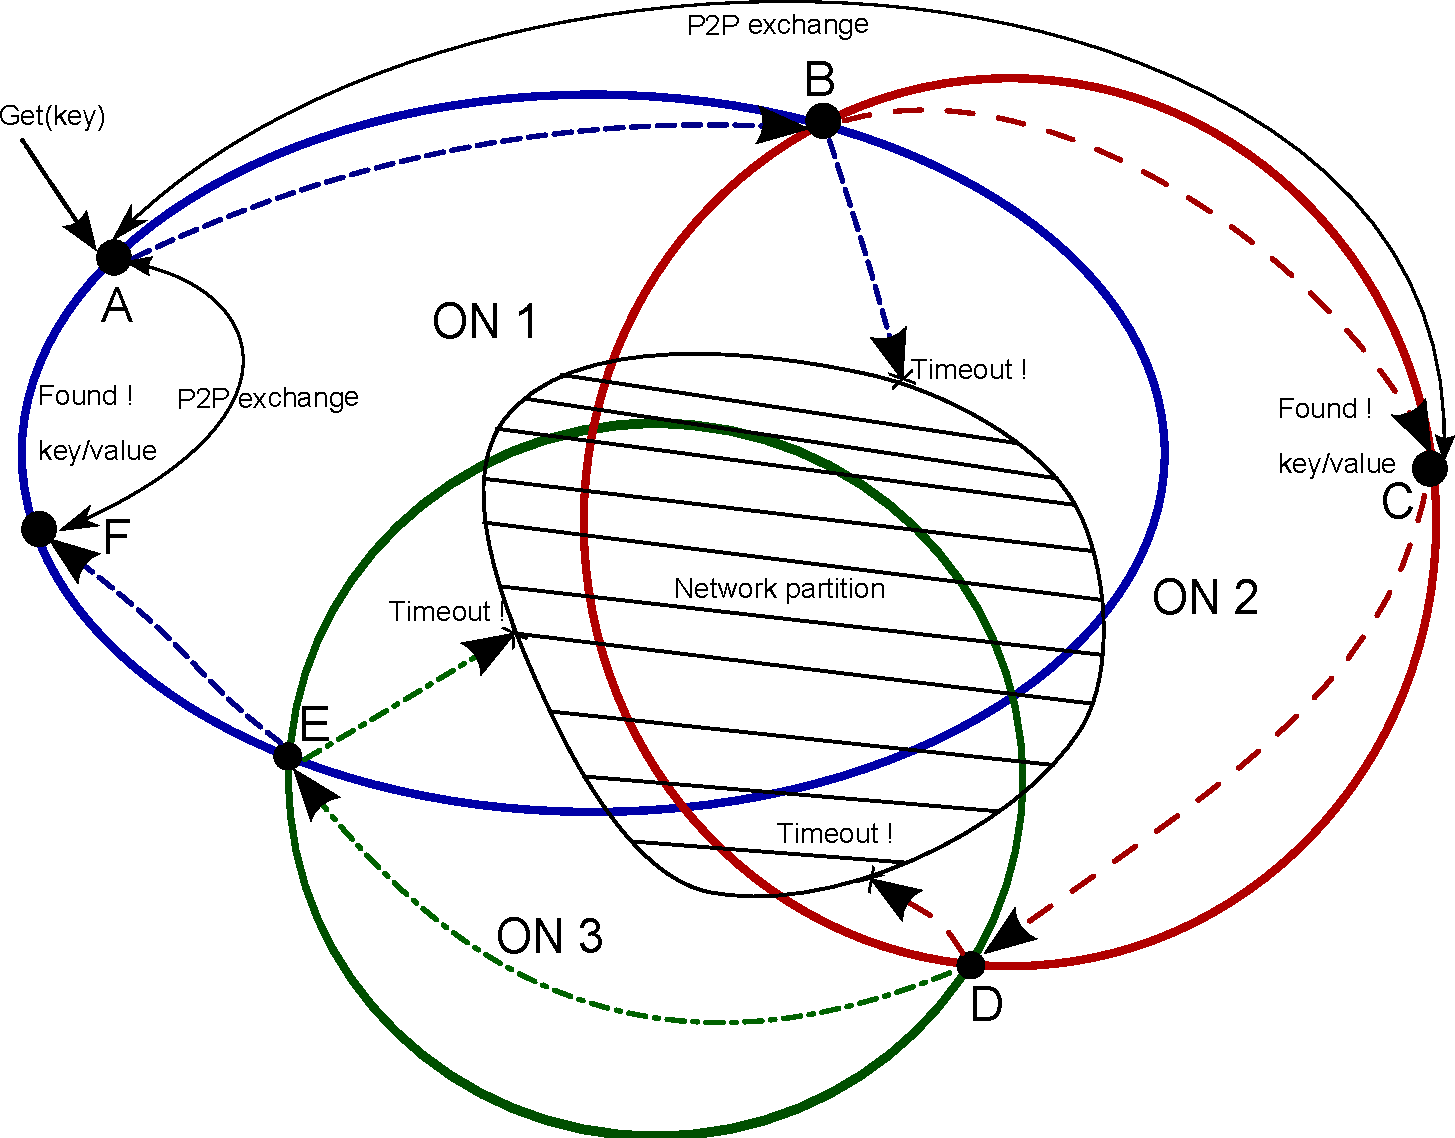
\includegraphics[width=0.6\columnwidth]{fig/ON_with_network_partition.pdf}
%   \caption{Dealing with a network partition\label{fig:example2}}
% \end{figure}
%
\begin{figure}[!t]
\up{4}
  \centering
  \mbox{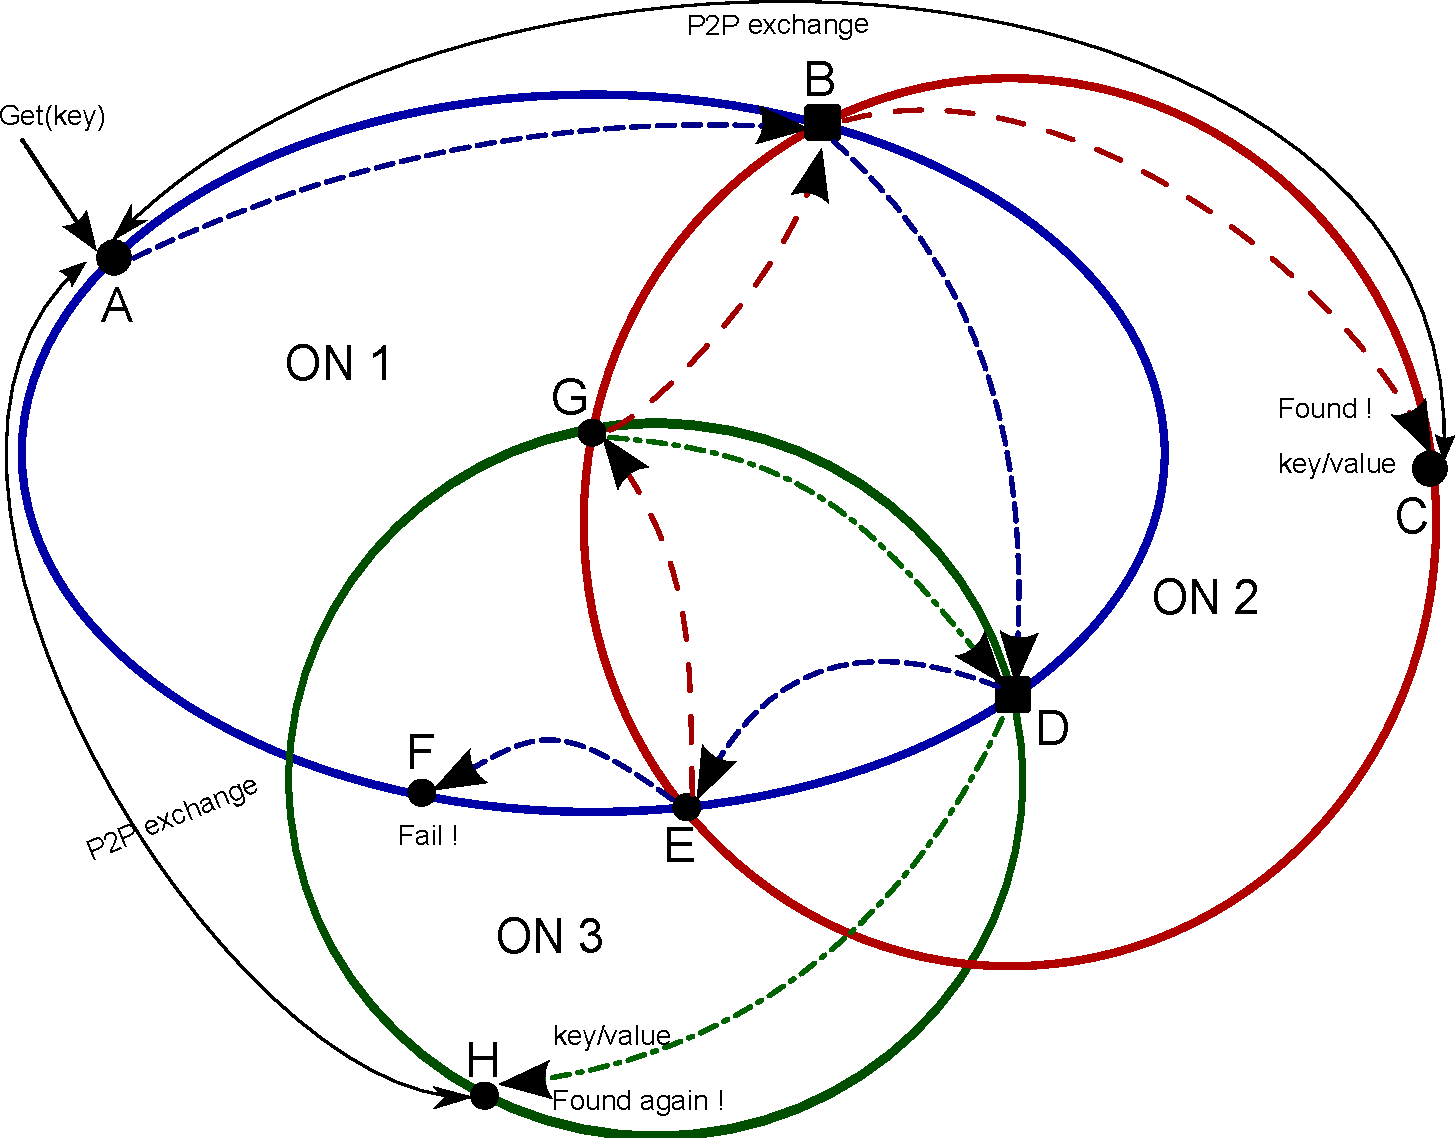
\includegraphics[width=0.5\columnwidth]{fig/GET_into_other_ON.pdf}\,\,
    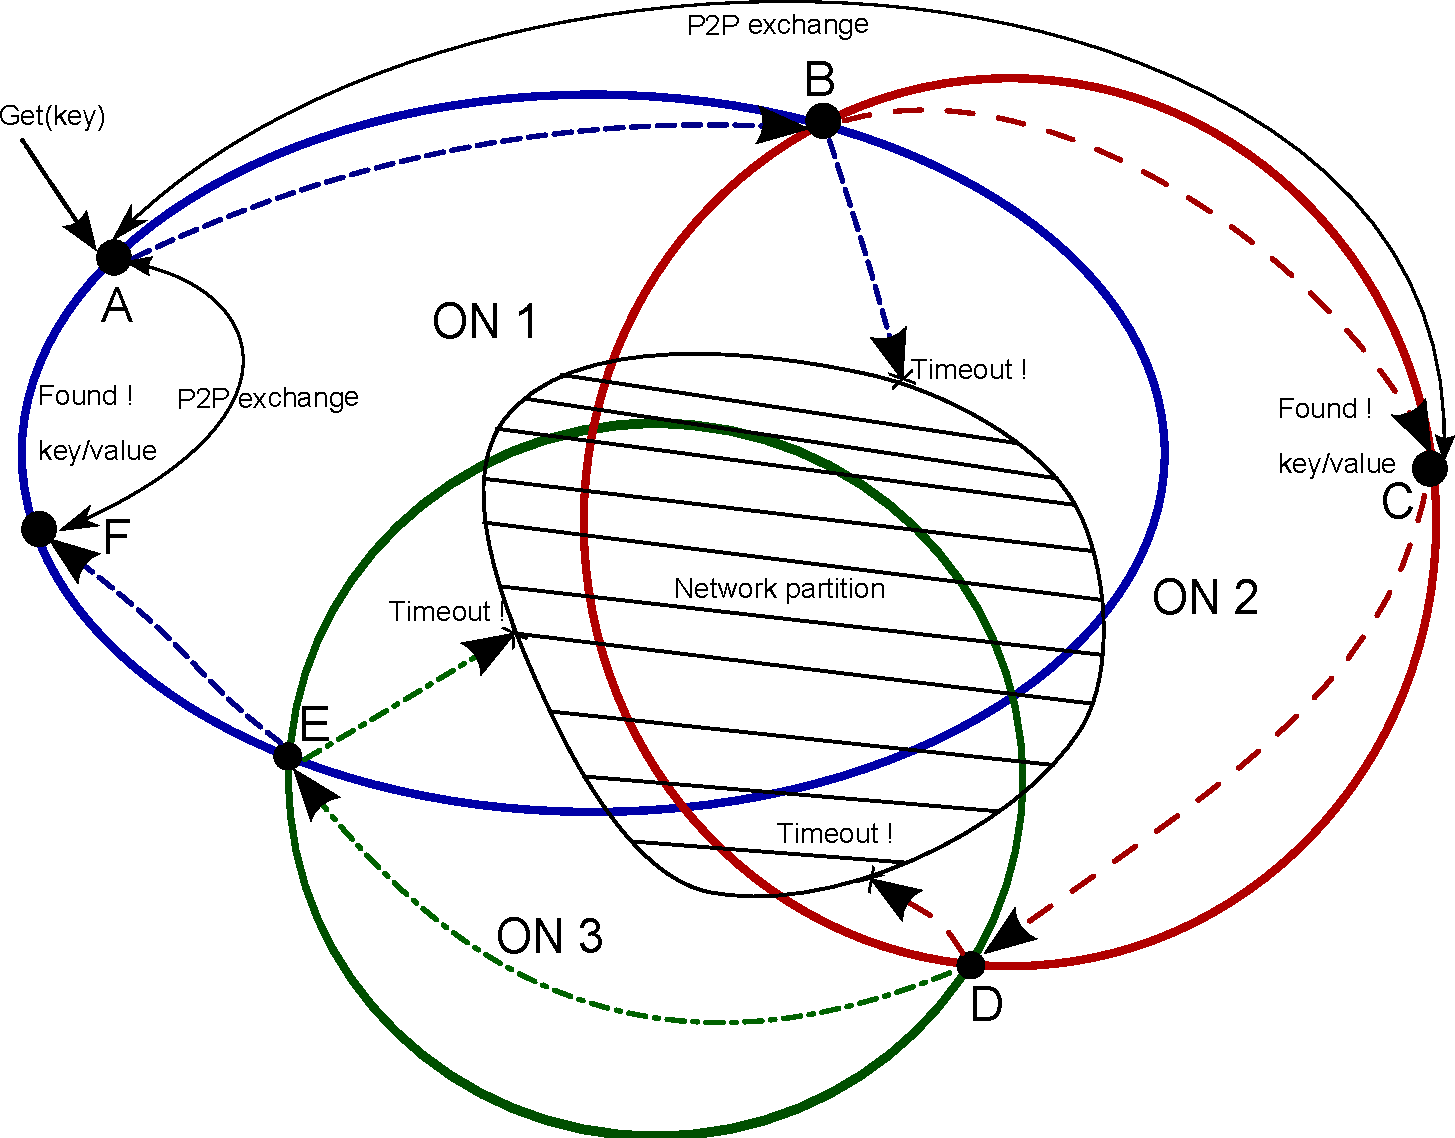
\includegraphics[width=0.5\columnwidth]{fig/ON_with_network_partition.pdf}}
  \caption{Routing across differents overlays and dealing with a network partition\label{fig:example}}
\up{8}
\end{figure}
%
%\subsection{Examples}
%
%\noindent {\bf Examples.} We illustrate the Synapse protocol by means
%of two examples.
% (From now on we denote {\tt FIND(GET/PUT)} simply by {\tt GET/PUT}).

% \begin{figure}
%   \centering
%   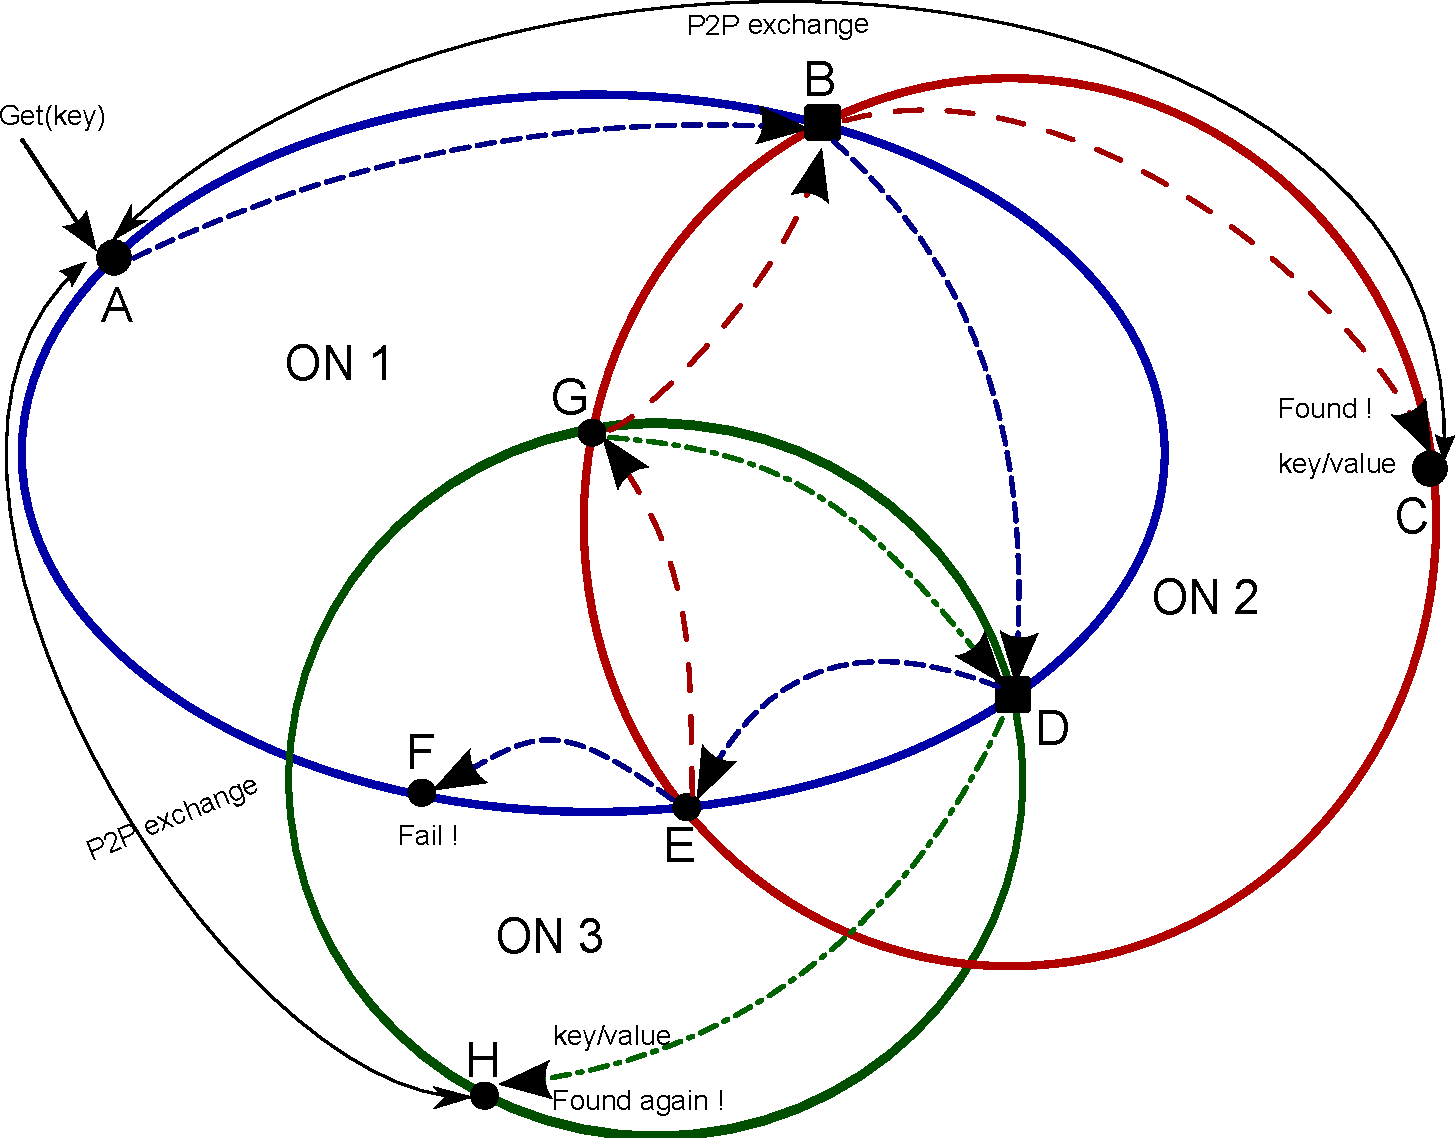
\includegraphics[width=0.6\columnwidth]{fig/GET_into_other_ON.pdf}
%  \caption{Routing across differents overlays \label{fig:example1}}
% \end{figure}

\noindent {\bf Example 1. Routing across differents intra-overlays.}
%
Figure \ref{fig:example} shows how a value present in one overlay can
be retrieved from a {\tt GET} launched by another overlay. Peer A in
the overlay ON1 receives a {\tt GET(key)} message: the routing goes
until the synapse B, which triggers a second intra-overlay routing in
ON2. The two routings proceed in parallel, and, in particular, the
routing in ON2 terminates successfully with a peer-to-peer interaction
between the peer A and peer C responsible of the resource. Routing
continues on ON1 until synapse D, which triggers a third
intra-overlay routing in ON3. The routing proceeds in parallel, and, in
particular, routing in ON3 terminates successfully with a second
peer-to-peer interaction between A and H, while routing in ON1
proceeds to a failure on peer F via the synapse E. Synapse E
launches a fourth intra-overlay routing in ON2 that proceeds to a
failure on node B (game over strategy) via synapse G. Finally, G
launches a fifth intra-overlay routing on ON3, terminating with a
failure on D (again game over strategy). Peers playing game over
strategy are depicted as squares.

\noindent {\bf Example 2. Dealing with network partition.}
%
Figure \ref{fig:example} also shows how intra-overlays take
advantage of joining each other in order to recover situations where
network partitioning occurs (because of the partial failure of nodes or the high
churn of peers). Since network partitions affect routing performance and
produce routing failures, the possibility of retrieving a value in a
failed intra-overlay routing is higher, thanks to alternative
inter-overlay paths. More precisely, the figure shows how a value
stored in peer E of the overlay ON1 can be retrieved in presence
of a generic network partition by routing via ON2 and ON3 through
synapses B,C,D, and E.  The reader can refer to the web appendix for
a detailed description of the protocol pseudocode, in both the white and
the black box model.

